% ViTALBench -- Springer LNCS version (converted from AAAI-27 submission)
\documentclass[runningheads]{llncs}
% Large embedded figure PDFs overflow pdfTeX's object stream buffer; disable object streams.
\pdfobjcompresslevel=0
%
\usepackage[T1]{fontenc}
\usepackage{newtxtext}
\usepackage[varvw]{newtxmath}   % also provides the AMS symbols (do not load amssymb)
%
\usepackage{amsmath}
\usepackage{graphicx}
\usepackage{booktabs}
\usepackage{pifont}             % \ding{51} / \ding{55}
\usepackage{xcolor}
\usepackage[nointegrals]{wasysym} % \LEFTcircle
\usepackage[hyphens]{url}
\usepackage{marvosym}
%
% Optional (Springer eBook style links):
%\usepackage{hyperref}
%\renewcommand\UrlFont{\color{blue}\rmfamily}
%\urlstyle{rm}

\begin{document}
%
\title{\textsc{ViTALBench}: A Vietnamese Traffic-Law Benchmark Dataset for Multimodal Legal Reasoning}
\titlerunning{\textsc{ViTALBench}: Vietnamese Traffic-Law Multimodal Benchmark}
%
% TODO: replace with the real author list.
\author{Dang Le\inst{1}\orcidID{0009-0002-9557-2636} \and
Duy-Minh Nguyen-Tran\inst{1}\orcidID{0000-0001-7626-5142} \and
Thinh-Hung Nguyen \inst{1}\orcidID{0000-0001-7626-5142} \and
Le-Minh Nguyen\inst{1}(\Letter)\orcidID{0000-0002-2265-1010}}
%
\authorrunning{Dang Le et al.}
%
\institute{Japan Advanced Institute of Science and Technology, Ishikawa, Japan\\
\email{\{lnhdang14, ntdminh, nguyenml\}@jaist.ac.jp}}


\maketitle
%
\begin{abstract}
Vision-language models (VLMs) have advanced rapidly, yet their ability to perform grounded multimodal legal reasoning remains underexplored. In traffic-law applications, this capability requires models to identify violations from visual evidence, link those observations to applicable legal provisions, and determine the corresponding legal consequences. However, existing traffic-oriented benchmarks typically evaluate visual scene understanding and traffic-law knowledge in isolation, leaving it unclear whether VLMs can translate visual evidence into legally valid decisions. To address this gap, we introduce \textsc{ViTALBench}, a multiple-choice visual question answering benchmark containing 4,536 questions, grounded in current Vietnamese traffic regulations.
\textsc{ViTALBench} contains two top-level tiers: detection and law. The law tier is divided into violation identification, regulation application, and multi-step legal reasoning, evaluating visual scene understanding and statute-dependent reasoning grounded in external legal knowledge. Across ten VLMs from three model families, we find a consistent performance gap between visual perception and legally grounded reasoning, with every model performing substantially worse on questions that require statutory grounding. Further analysis shows that the main bottlenecks are not visual perception alone, but limited statutory knowledge and difficulty integrating legal text with visual evidence to produce legal conclusions.
The dataset is available at \url{https://anonymous.4open.science/r/ViTAL_BENCH-BB6C/}.

\keywords{Vision-language models \and Multimodal legal reasoning \and Traffic law \and Visual question answering \and Benchmark.}
\end{abstract}

\section{Introduction}
\begin{figure}[t]
\centering
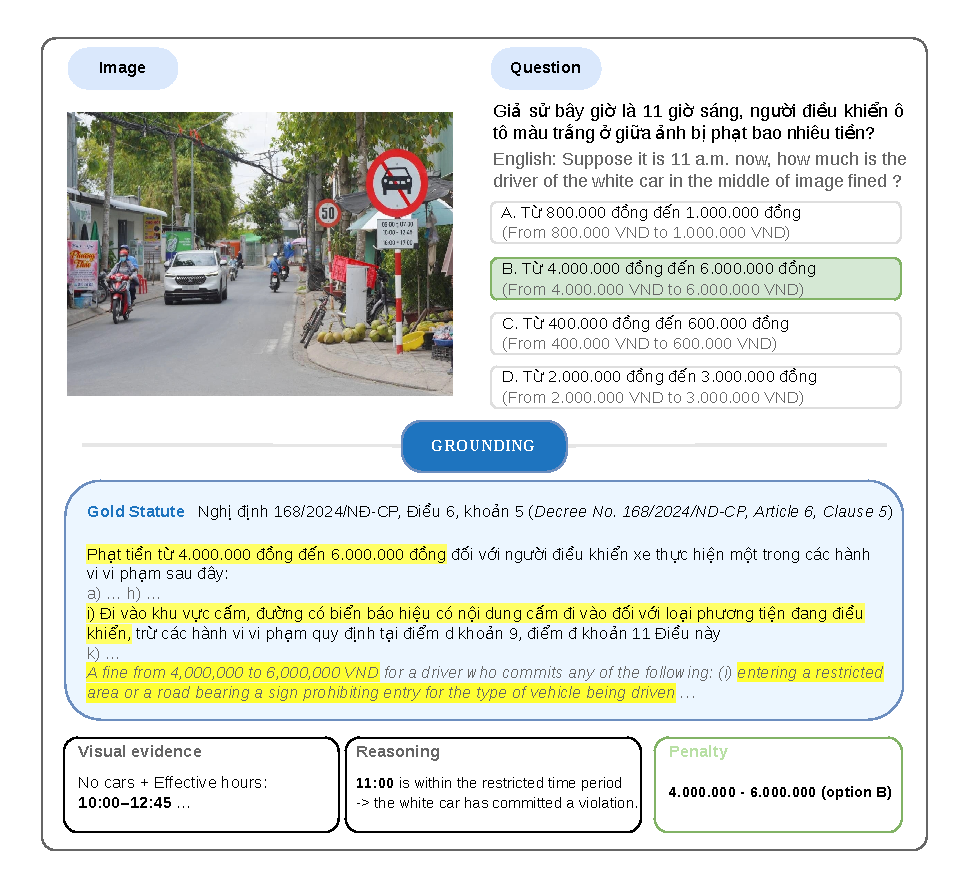
\includegraphics[width=\linewidth]{Figures/Sample2.pdf}
\caption{
An example from \textsc{ViTALBench}. The grounding shown is provided only for illustration and is not part of the benchmark annotations.
}
\label{fig:sample}
\end{figure}
Recent advances in vision-language models (VLMs)  have significantly enhanced their ability to perceive and reason about complex traffic environments~\cite{zhou2024vision}. Nevertheless, recognizing a traffic violation is fundamentally different from understanding a traffic scene. It requires reasoning beyond visual recognition. A model must understand the traffic context, identify potential violations, link its judgment to relevant legal provisions, and determine the associated legal consequences. Despite impressive progress in intelligent transportation tasks~\cite{li2023blip,liu2024improved,wang2024qwen2,chen2023internvl,wu2025trafficinternvl,kuang2025traffic}, existing VLMs have rarely been evaluated on this integrated perception and legal reasoning capability. Bridging this gap is crucial for building trustworthy AI systems that can support traffic law enforcement and legal decision-making.

To support research in intelligent transportation, several traffic-oriented vision-language benchmarks have been introduced~\cite{qian2024nuscenesqa,wei2025driveqa,guan2026roadscenevqa,luu2025vlsp}. These benchmarks have significantly advanced the evaluation of traffic scene understanding, driving knowledge, behavior analysis, and traffic rule comprehension. However, they primarily focus on perceptual understanding or traffic-related knowledge, without assessing whether models can transform visual evidence into legally grounded decisions. Beyond traffic-oriented benchmarks, legal reasoning benchmarks, including LexGLUE, LegalBench, LawBench, and recent multilingual legal reasoning datasets, have explored the ability of language models to understand and apply legal knowledge~\cite{chalkidis2022lexglue,guha2023legalbench,fei2024lawbench,yu2027benchmarking}. However, these benchmarks are predominantly text-based and do not capture the multimodal nature of real-world legal reasoning, where legal conclusions often depend on visual evidence. Therefore, a benchmark integrating visual evidence and legal decision-making remains unexplored. It leaves an open question whether modern vision-language models can derive legally grounded decisions from real-world traffic scenarios.


To address this gap, we introduce \textsc{ViTALBench}, a benchmark for evaluating legally grounded multimodal reasoning in traffic scenarios. \textsc{ViTALBench} is built upon current Vietnamese traffic regulations, whose fine-grained, behavior-dependent penalties provide a realistic and practically relevant testbed for legal reasoning. Although instantiated using Vietnamese law, the task formulation is general and can be readily adapted to other jurisdictions. We construct the benchmark through a multi-stage annotation pipeline that integrates LLM-assisted question generation with human verification. Specifically, questions are generated from real-world traffic images and validated by native-speaker annotators against official legal documents, ensuring that each sample and legal citation is grounded in verified evidence. The released benchmark contains 4,536 multiple-choice questions over 551 images in 11 categories. It includes 2,122 detection questions and 2,414 law questions, with the law tier divided into violation identification, regulation application, and multi-step legal reasoning.

Using \textsc{ViTALBench}, we evaluate ten open VLMs under a unified evaluation protocol. Our analysis reveals a consistent gap between visual understanding and legal reasoning across all models. While visual perception performance is relatively strong, accuracy drops substantially once models must identify the applicable regulation and infer the corresponding legal consequences. Even the best-performing model achieves only 67.4\% accuracy on statute-dependent legal reasoning without access to the relevant legal documents. These results highlight the limitations of current VLMs in regulation-grounded reasoning and underscore the need for further advances before they can be reliably deployed in safety-critical transportation applications.

Our main contributions are summarized as follows:

\begin{itemize}

\item We introduce \textbf{\textsc{ViTALBench}}, to the best of our knowledge, the first benchmark for evaluating legally grounded multimodal reasoning from visual evidence in traffic scenarios.

\item We develop a human-verified benchmark comprising 4,536 multiple-choice questions over 551 traffic images, with detection and law tiers and three law-reasoning categories.

\item We evaluate ten representative vision-language models and conduct detailed analyses of their capabilities and limitations, revealing substantial gaps between visual understanding and regulation-grounded legal reasoning.

\end{itemize}


\section{Related Work}
\begin{table}[t]
\centering
\caption{Comparison of \textsc{ViTALBench} with representative traffic and legal reasoning benchmarks. \textcolor{green}{\ding{51}} indicates full support, $\LEFTcircle$ partial support, and \textcolor{red}{\ding{55}} indicates no support. \textit{Perception} denotes understanding of visual traffic scenes; \textit{Violation Identification} refers to detecting traffic violations from observations; \textit{Regulation Application} indicates whether models can apply relevant traffic rules; \textit{Multi-step Legal Reasoning} measures reasoning over multiple legal steps; and \textit{Grounded in Real Legal Code} indicates whether decisions are supported by official legal regulations.}
\label{tab:benchmark_comparison}
\setlength{\tabcolsep}{3pt}
\resizebox{\textwidth}{!}{%
\begin{tabular}{lccccccc}
\toprule
\textbf{Benchmark} &
\textbf{Year} &
\textbf{Modality} &
\textbf{Perception} &
\textbf{Violation} &
\textbf{Regulation} &
\textbf{Multi-step} &
\textbf{Grounded in} \\
&
&
&
&
\textbf{Identification} &
\textbf{Application} &
\textbf{Legal Reasoning} &
\textbf{Real Legal Code} \\
\midrule
LexGLUE       & 2022 & Text & \textcolor{red}{\ding{55}} &  \textcolor{red}{\ding{55}} & \textcolor{green}{\ding{51}} & $\LEFTcircle$ & \textcolor{green}{\ding{51}} \\
LegalBench    & 2023 & Text &  \textcolor{red}{\ding{55}} &  \textcolor{red}{\ding{55}} & \textcolor{green}{\ding{51}} & \textcolor{green}{\ding{51}} & \textcolor{green}{\ding{51}}\\
LawBench    & 2024 & Text &  \textcolor{red}{\ding{55}}&  \textcolor{red}{\ding{55}}& \textcolor{green}{\ding{51}}& \textcolor{green}{\ding{51}} & \textcolor{green}{\ding{51}}\\
NuScenes-QA  & 2024 & Image+Text &\textcolor{green}{\ding{51}}&  \textcolor{red}{\ding{55}}&  \textcolor{red}{\ding{55}} & \textcolor{green}{\ding{51}}&  \textcolor{red}{\ding{55}} \\
DriveQA      & 2025 & Image+Text & \textcolor{green}{\ding{51}} &  \textcolor{red}{\ding{55}} & $\LEFTcircle$ & \textcolor{green}{\ding{51}}&  \textcolor{red}{\ding{55}}\\
MLQA-TSR     & 2025 & Image+Text & $\LEFTcircle$ &  \textcolor{red}{\ding{55}} & \textcolor{green}{\ding{51}} &  \textcolor{red}{\ding{55}} & \textcolor{green}{\ding{51}}\\
RoadSceneVQA & 2026 & Image+Text & \textcolor{green}{\ding{51}}& $\LEFTcircle$ &  \textcolor{red}{\ding{55}} & $\LEFTcircle$ &  \textcolor{red}{\ding{55}} \\
\midrule
\textbf{\textsc{ViTALBench}} & \textbf{2026} & Image+Text &
\textcolor{green}{\ding{51}}&
\textcolor{green}{\ding{51}}&
\textcolor{green}{\ding{51}} &
\textcolor{green}{\ding{51}}&
\textcolor{green}{\ding{51}}\\

\bottomrule
\end{tabular}}
\end{table}
Recent advances in VLMs have led to a series of multimodal benchmarks for intelligent transportation systems. Existing traffic-oriented benchmarks mainly evaluate three complementary capabilities: traffic scene understanding, driving situation reasoning, and traffic regulation comprehension. NuScenes-QA~\cite{qian2024nuscenesqa} focuses on traffic scene perception through question answering about objects, road layouts, and driving context. DriveQA~\cite{wei2025driveqa} extends this setting by incorporating traffic regulation knowledge into driving-related reasoning. RoadSceneVQA~\cite{guan2026roadscenevqa} introduces violation-related questions grounded in traffic scenes, although it does not systematically connect identified violations to specific legal provisions. MLQA-TSR~\cite{luu2025vlsp} instead emphasizes traffic sign recognition based on regulatory documents without evaluating violation identification or legal consequence prediction. Although these benchmarks have substantially advanced multimodal reasoning for intelligent transportation, they mainly evaluate visual understanding and driving knowledge rather than legally grounded decision-making. In most cases, models are not required to explicitly identify the governing legal provision or justify their predictions using statutory evidence. Consequently, strong performance on existing traffic benchmarks does not necessarily indicate that a model can perform regulation-grounded legal reasoning in real-world traffic scenarios.

In parallel, legal reasoning has emerged as an important research direction with the rise of large language models. Existing legal benchmarks, including LexGLUE~\cite{chalkidis2022lexglue}, LegalBench~\cite{guha2023legalbench}, and LawBench~\cite{fei2024lawbench}, focus on legal reasoning over textual statutes, case documents, and legal knowledge. While these benchmarks provide valuable evaluations of language-based legal reasoning, they assume that all relevant evidence is explicitly available in text. This assumption differs fundamentally from traffic law enforcement, where the primary evidence is visual, and the applicable legal provision must first be inferred from the observed scene. Consequently, success on textual legal reasoning benchmarks does not imply the ability to perform multimodal legal reasoning grounded in visual evidence.

These observations highlight an important distinction between traffic regulation comprehension and regulation grounding. The former only requires benchmarks to incorporate regulatory knowledge, whereas the latter requires models to identify violations and justify their decisions based on the specific legal provisions governing observed behaviors. Existing benchmarks largely evaluate these capabilities separately and do not assess the complete reasoning process that connects visual evidence to legally justified decisions. As summarized in Table~\ref{tab:benchmark_comparison}, \textsc{ViTALBench} bridges this gap by jointly evaluating visual perception, violation identification, regulation application, and multi-step legal reasoning, with each benchmark instance grounded in real legal codes.


\section{\textsc{ViTALBench} Dataset}
\label{sec:dataset}
\begin{figure}[t]
\centering
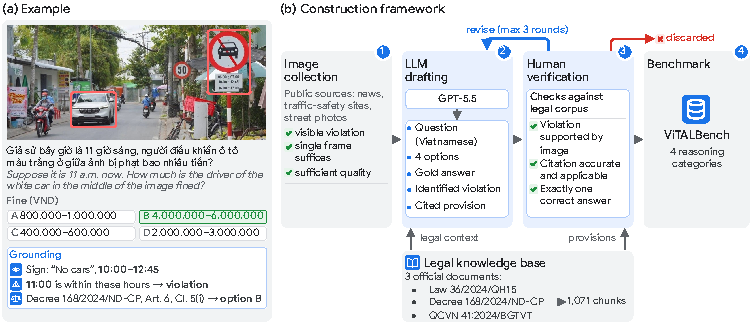
\includegraphics[width=\textwidth]{Figures/Model.pdf}
\caption{Overview of the \textsc{ViTALBench} construction pipeline. Starting from real-world traffic images, an LLM generates candidate question-answer pairs and associated legal information, which are subsequently verified and refined by human annotators against official Vietnamese traffic regulations to produce the final benchmark.}
\label{fig:pipeline}
\end{figure}

\textsc{ViTALBench} is constructed through a multi-stage pipeline that combines LLM-assisted annotation with human verification against official Vietnamese traffic regulations. As illustrated in Figure~\ref{fig:pipeline}, the pipeline consists of image collection, candidate question generation, manual verification, and benchmark curation.

\subsection{Dataset Construction}
\paragraph{Data collection.}
To ensure broad coverage, we first define a set of common violation categories based on current Vietnamese traffic regulations and search for images corresponding to each category. Images are collected from publicly accessible online sources, including news articles, traffic-safety websites, and publicly shared street photographs. Because traffic regulations vary across countries, \textsc{ViTALBench}  only focuses on scenarios governed by Vietnamese law. We retain only images that satisfy three criteria: \textbf{(1)} at least one traffic violation is visually identifiable; \textbf{(2)} the violation can be determined from a single frame, without temporal information; and \textbf{(3)} image quality is sufficient to recognize the relevant traffic participants and infrastructure. Duplicate and visually redundant images are removed during curation.

The resulting collection contains 551 images captured from diverse viewpoints, including street-level photographs and road cameras. It covers urban roads, intersections, residential streets, and highways, and includes motorcycles, passenger vehicles, buses, trucks, and pedestrians. All images are collected exclusively from publicly accessible sources for research purposes. Personally identifiable information, including visible faces and vehicle license plates, is anonymized or obscured when necessary to reduce privacy risks.

\paragraph{Legal knowledge base.}
We construct a legal knowledge base from three official documents governing road traffic in Vietnam. These include the National Technical Regulation on Road Signs and Signals, QCVN 41:2024/BGTVT, the Law on Road Traffic Order and Safety, Law No. 36/2024/QH15, and Decree No. 168/2024/ND-CP on administrative penalties for road traffic violations. Each document is segmented at the article level while preserving the document name, article identifier, and original legal text, resulting in 990 chunks. This organization allows annotators to retrieve and verify the provisions governing each observed violation and its corresponding legal consequences.

\paragraph{Hybrid human-AI annotation.}
Constructing legally grounded questions at scale requires both efficient generation and careful legal verification. LLMs can rapidly draft fluent questions and plausible distractors, but they may produce inaccurate citations or unsupported legal interpretations. Manual authoring alone, however, is costly and difficult to scale across thousands of questions and multiple legal documents. We therefore adopt a two-stage annotation protocol in which an LLM generates candidate instances and human annotators verify them against the legal knowledge base.
\paragraph{Stage 1. LLM drafting.}
GPT-5.5 is provided with the relevant legal context and used to generate initial instances for each image. Each draft contains a multiple-choice question, candidate answer options, the correct answer, the identified violation, and a reference to the potentially applicable legal provision. The model is instructed to produce distractors that are plausible within the traffic context but legally incorrect. All outputs are treated as preliminary drafts rather than final annotations.
\paragraph{Stage 2. Human verification against the legal corpus.}
Because a model may cite a provision that does not exist or does not apply, every draft is subsequently verified by a human annotator against the legal corpus. The annotator uses the identified violation and proposed citation as retrieval queries, reads the retrieved provisions, and checks three conditions. The identified violation must be fully supported by the visual evidence. The cited regulation must be legally accurate and applicable to the observed scenario. The question and answer options must be clear, legally unambiguous, and contain exactly one correct answer. When an instance fails any of these checks, the annotator provides the retrieved statutory evidence and revision instructions to the LLM. The revised instance is then verified again. This refinement process is limited to three rounds. Items that remain invalid or ambiguous after three rounds are removed. Samples are also discarded when they contain unsupported violations, incorrect legal references, or errors that cannot be reliably corrected.
\paragraph{Annotation quality assessment.}
To assess annotation reliability, we randomly sample 300 questions for independent human verification. Two experts knowledgeable in Vietnamese traffic regulations independently evaluate each question with respect to violation identification, statutory grounding, legal consequences, and answer correctness. The resulting agreement rate is $96.1\%$, with Cohen's $\kappa$ of $0.88$, indicating strong inter-annotator agreement. All disagreements are resolved through discussion before the final annotations are produced.

\paragraph{Reasoning taxonomy.}


Prior traffic VQA benchmarks distinguish between explicit scene perception and higher-level context-aware reasoning about traffic behavior and compliance. Building on this distinction, \textsc{ViTALBench} introduces a finer-grained taxonomy that decomposes legally grounded traffic reasoning into four categories with increasing dependence on statutory knowledge.


\begin{itemize}
    \item \textbf{Visual Perception.}
    These questions assess whether a model can recognize traffic-related elements directly observable in the image, including traffic signs, signals, lane markings, road layouts, vehicle types, participant positions, and visible behaviors. They require visual-semantic grounding but do not require a legal judgment.


    \item \textbf{Violation Identification.}
    These questions require the model to determine whether the observed behavior constitutes a traffic violation. Unlike visual perception, this category requires combining multiple scene cues, such as participant behavior, signal state, road structure, and surrounding context, to reach a compliance judgment. However, the model is not required to identify the specific governing provision or legal consequence.

    \item \textbf{Regulation Application.}
    These questions assume that the relevant behavior or violation has been identified and require the model to apply the corresponding statutory provision. The expected answer may concern the applicable fine, license-point deduction, license suspension, or another legal consequence. This category, therefore, evaluates whether a model can move from a recognized violation to a legally grounded decision.


    \item \textbf{Multi-step Legal Reasoning.}
    These questions require the complete reasoning process from visual evidence to legal consequence. A model must identify the relevant traffic participants and contextual cues, determine the violation, apply applicable legal conditions or exceptions, and select the final answer based on one or more statutory provisions. This category captures scenarios in which the legal conclusion depends on several interdependent visual and statutory conditions.

\end{itemize}



\subsection{Dataset Statistics}

\begin{figure}[t]
\centering
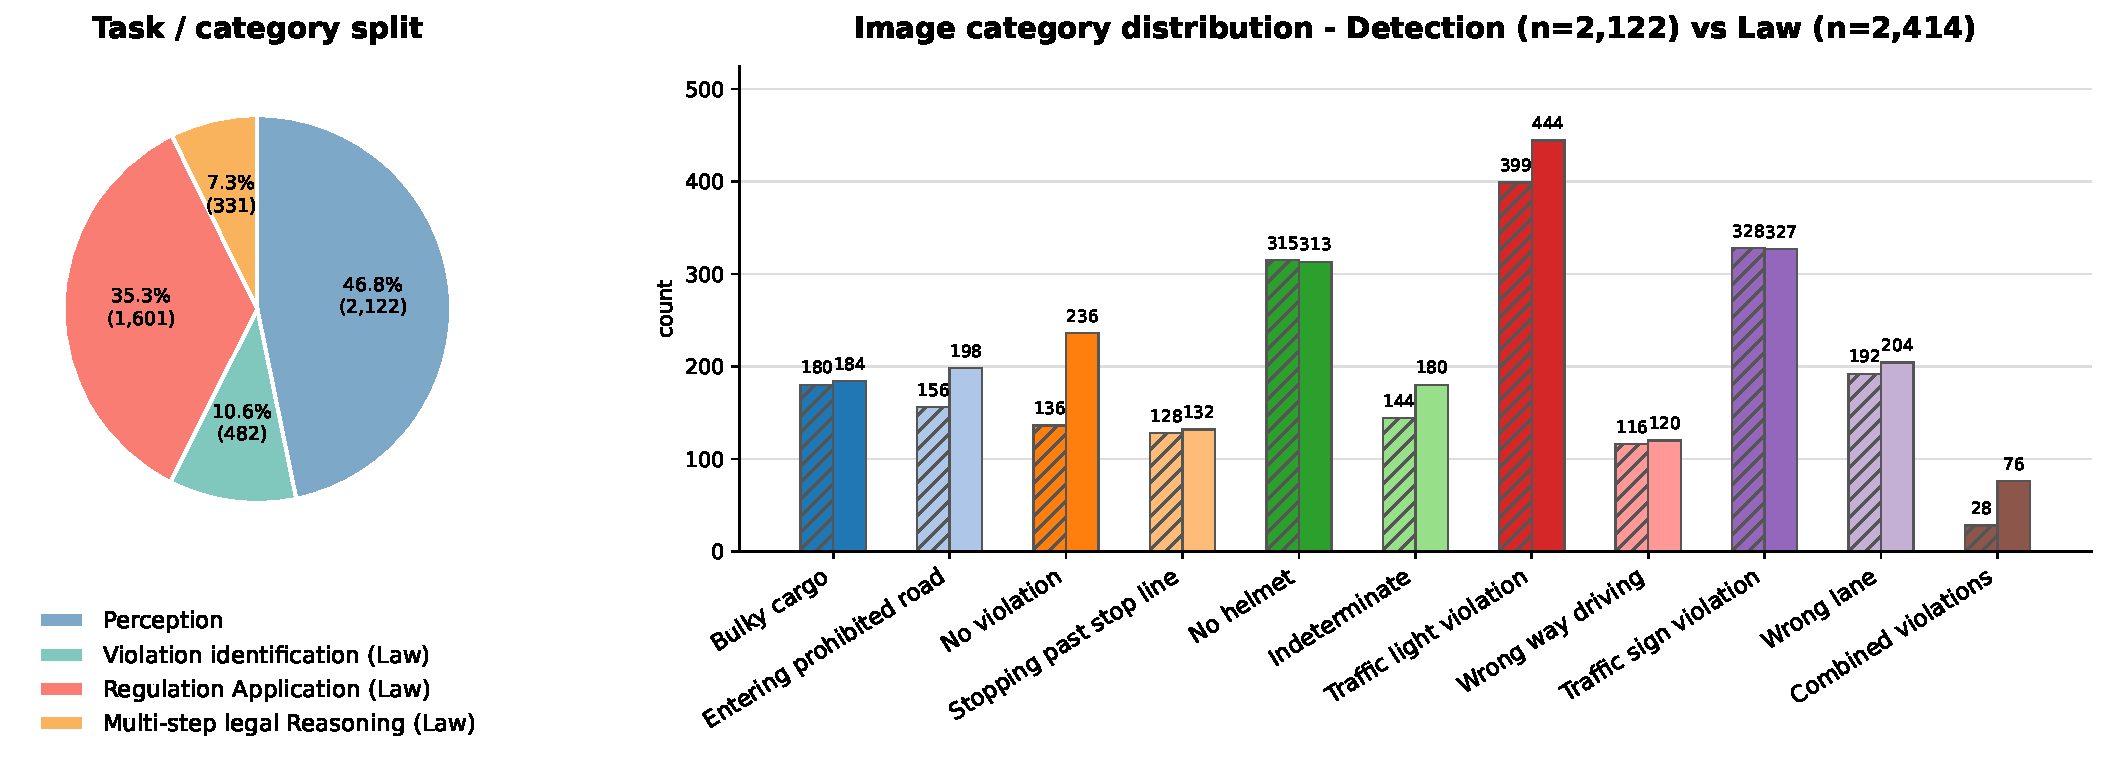
\includegraphics[width=\textwidth]{Figures/Statistic.pdf}
\caption{Statistics of \textsc{ViTALBench}.}
\label{fig:statistic}
\end{figure}

Figure~\ref{fig:statistic} summarizes the statistics of \textsc{ViTALBench}. The release contains 4,536 multiple-choice questions over 551 images in 11 categories, including 2,122 detection questions and 2,414 law questions. The law questions comprise 482 Violation Identification questions, 1,601 Regulation Application questions, and 331 Multi-step Legal Reasoning questions. The accompanying release audit script computes these counts from the canonical files `datasets/questions/detection.json`, `datasets/questions/law.json`, `datasets/legal/law_categories.json`, and `datasets/legal/law_db.json`.

To reflect realistic traffic law enforcement scenarios, \textsc{ViTALBench} covers a broad spectrum of traffic violations rather than focusing on only a few frequently occurring cases. These include traffic-sign violations, lane usage, helmet regulations, speeding, illegal stopping and parking, wrong-way driving, vehicle loading, and other regulation-dependent behaviors. In addition, some benchmark instances contain multiple concurrent violations, requiring models to integrate multiple visual cues before determining the applicable regulation and legal consequence.

The reasoning-category distribution is intentionally imbalanced to better reflect the frequency and complexity of real-world traffic enforcement scenarios. Perception and Regulation Application account for approximately 80\% of the benchmark because these reasoning stages naturally arise in most traffic-law cases, whereas Multi-step Legal Reasoning represents comparatively rarer but substantially more complex scenarios. To mitigate the effects of this imbalance, we report both overall performance and category-wise accuracy in our experiments, enabling fair evaluation across different reasoning levels.

\section{Experiments and Analysis}
\label{sec:experiments}

\paragraph{Overview.}
We conduct a series of experiments to identify the capabilities and limitations of modern VLMs on \textsc{ViTALBench}. Our analysis is organized around four research area questions:

\begin{itemize}
\item \textbf{RQ1.} How does model performance change as questions move from visual scene understanding to increasingly statute-dependent legal reasoning?

\item \textbf{RQ2.} To what extent can statutory evidence close the
performance gap between perception and legal reasoning?

\item \textbf{RQ3.} Are models aware of their own knowledge gaps, abstaining
more when a question requires statutory grounding?
\item \textbf{RQ4.} How does model capacity affect the ability to leverage supplied statutory evidence?

\end{itemize}


\subsection{Experimental Setting}

\paragraph{Dataset.}
We conduct experiments on \textsc{ViTALBench} to evaluate the visual and legal reasoning capabilities of current VLMs. \textsc{ViTALBench} comprises a detection tier (\textbf{Detection}; 2{,}122 items) and a legal tier (2{,}414 items) split by the reasoning it demands: \textbf{Violation Identification} (482), \textbf{Regulation Application} (1{,}601), and \textbf{Multi-step Legal Reasoning} (331). All legal questions are grounded in current Vietnamese traffic regulations.

\paragraph{Models.}
We evaluate ten open VLMs from four model families and across a broad range of parameter scales. These include InternVL3 \cite{zhu2025internvl3exploringadvancedtraining} with 1B, 2B, 8B, and 14B parameters, Qwen3-VL-Instruct \cite{bai2025qwen3vltechnicalreport} with 2B, 4B, and 8B parameters, Qwen2.5-VL \cite{bai2025qwen25vltechnicalreport} with 3B and 7B parameters, and Llama-3.2-11B-Vision \cite{touvron2023llamaopenefficientfoundation}.

\paragraph{Configuration and metrics.}
All models are evaluated in BF16 on a single NVIDIA A100 40 GB GPU using identical prompts and inference settings. We report multiple-choice accuracy under two evaluation protocols. The 4-option protocol contains only the four candidate answers, whereas the 5-option protocol adds an explicit \textit{Not sure} option, allowing models to abstain rather than select one of the content answers.

% ============================================================
\section{Analysis Results}
\label{sec:results}

% ------------------------------------------------------------
\subsection{A large gap separates perception from legal reasoning}
\label{sec:gap}
\paragraph{Experiments.} To examine how performance changes as questions progress from visual scene understanding to increasingly statute-dependent legal reasoning, all ten VLMs are evaluated under the 4-option protocol. Accuracy is reported in Table~\ref{tab:pertype} separately for Perception, Violation Identification, Regulation Application, and Multi-step Legal Reasoning. The average across the three legal categories is also reported as the overall legal-tier accuracy.
\paragraph{Analysis.}
All ten models perform substantially better on Perception than on the legal tier. Across models, average accuracy falls from $83.5\%$ on Perception to $60.1\%$ on legal questions, producing a consistent gap of $23.4$ percentage points. This gap shows that strong visual understanding does not necessarily translate into legally grounded decisions.

Performance generally declines as questions become more dependent on statutory knowledge. Average accuracy decreases from $68.7\%$ on Violation Identification to $58.9\%$ on Regulation Application and $53.3\%$ on Multi-step Legal Reasoning. Models can often identify a violation from visible behavior, but they struggle when required to determine the governing provision, apply relevant legal conditions, and infer the corresponding consequences. The main difficulty, therefore, emerges when models must move beyond recognizing a traffic event and ground their decisions in specific legal rules. Increasing model size does not consistently close this gap. Within InternVL3, scaling from 1B to 14B reduces the gap between Perception and Violation Identification from $19.1$ to $1.9$ points, while increasing the gap between Perception and Regulation Application from $15.8$ to $29.3$ points. Qwen3-VL shows a similar pattern from 2B to 8B, with Violation Identification improving by $15.1$ points but Regulation Application by only $7.9$ points. Overall, scaling substantially improves visual understanding and violation recognition, but does not reliably improve the ability to interpret and apply the relevant law.

\begin{table}[t]
\centering
\caption{Accuracy (\%) by question type (4-option protocol). Every model is far stronger on Perception than on the legal tier, and within the legal tier, it drops most in Regulation Application and Multi-step Reasoning. Column maxima in bold. $^{\dagger}$Item-weighted average over the three legal types.}
\label{tab:pertype}
\setlength{\tabcolsep}{6pt}
\begin{tabular}{lccccc}
\toprule
Model & Perception & Vio.\,ID & Reg.\,App & Multi & Legal$^{\dagger}$ \\
& $\uparrow$ & $\uparrow$ & $\uparrow$ & $\uparrow$ & $\uparrow$ \\
\midrule
InternVL3-1B  & 74.3 & 55.2 & 58.5 & 53.8 & 57.2 \\
InternVL3-2B  & 80.9 & 49.6 & 53.3 & 45.3 & 51.5 \\
InternVL3-8B  & 89.2 & 80.1 & 63.5 & 60.7 & 66.4 \\
InternVL3-14B & \textbf{91.3} & \textbf{89.4} & 62.0 & 61.9 & 67.4 \\
Qwen3-VL-2B   & 81.6 & 64.9 & 55.9 & 45.3 & 56.3 \\
Qwen3-VL-4B   & 88.1 & 82.0 & 59.8 & 59.2 & 64.2 \\
Qwen3-VL-8B   & 89.6 & 80.1 & \textbf{63.8} & \textbf{62.5} & 66.9 \\
Qwen2.5-VL-3B & 81.7 & 73.9 & 54.5 & 49.2 & 57.7 \\
Qwen2.5-VL-7B & 85.4 & 67.2 & 56.6 & 49.8 & 57.8 \\
Llama-3.2-11B & 72.9 & 45.0 & 61.4 & 44.7 & 55.8 \\
\midrule
Average
& 83.5
& 68.7
& 58.9
& 53.3
& 60.1 \\
\bottomrule
\end{tabular}
\end{table}

% ------------------------------------------------------------
\subsection{Gold statutory evidence recovers much of the legal performance gap}
\label{sec:oracle}

\paragraph{Experiments.}
We examine whether the lower legal-tier performance is primarily associated with limited access to the governing law. For each legal question, we provide the model with the gold statutory provision at inference time and evaluate it under the \textsc{Legal}$_{+\text{gold}}$ setting. We compare this result with the original legal-tier accuracy obtained without external evidence. The Figure~\ref{fig:gold} presents the comparison for all ten models.


\paragraph{Analysis.}
Providing the governing provision improves legal accuracy for every model. The average gain is $14.2$ percentage points, with improvements ranging from $2.9$ points for InternVL3-1B to $18.8$ points for InternVL3-14B. InternVL3-14B improves from $67.4\%$ to $86.2\%$, while Qwen3-VL-8B increases from $66.9\%$ to $85.5\%$. Qwen3-VL-4B and Qwen2.5-VL-7B also show substantial gains of $18.0$ and $18.2$ points, respectively.

\begin{figure}[t]
\centering
    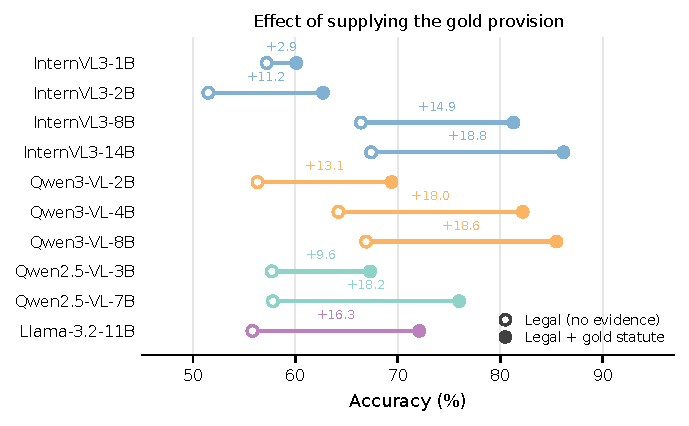
\includegraphics[width=\linewidth]{Figures/fig_gold_evidence.pdf}
\caption{Effect of supplying the governing statutory provision at inference.}
\label{fig:gold}
\end{figure}
The magnitude of improvement varies considerably across models. InternVL3-1B gains only $2.9$ points, whereas the larger InternVL3 models gain between $14.9$ and $18.8$ points. A similar pattern appears within Qwen3-VL, where the 2B model gains $13.1$ points but remains below the 4B
and 8B models after receiving the same gold evidence. These results indicate that limited access to statutory knowledge is a major source of error, but providing the correct provision does not guarantee successful legal reasoning. Models must still interpret the provision, connect its conditions to the visual evidence, and derive the appropriate legal consequence. The results, therefore,
highlight two complementary challenges: access to relevant statutory evidence and the ability to use that evidence effectively.



% ------------------------------------------------------------
\subsection{Abstention increases on statute-dependent questions}
\label{sec:abstain}
We next examine whether models express greater uncertainty when questions require statutory grounding. We extend the original 4-option protocol by adding a fifth option, \textit{Not sure}, allowing models to abstain rather than select one of the content answers. We measure the percentage of questions for which each model selects this option and report the results separately for Perception, Violation Identification, Regulation Application, and Multi-step Legal Reasoning in Table~\ref{tab:abstention}.


\paragraph{Analysis.}
Models abstain much more frequently on questions that require statutory knowledge. Across all models, the mean abstention rate is only $2.3\%$ for Perception and $3.8\%$ for Violation Identification. However, it increases to $25.0\%$ for Regulation Application and $21.9\%$ for Multi-step Legal Reasoning. Models, therefore, select \textit{Not sure} nearly eight times more often on the two statute-dependent categories than on the two categories that rely primarily on visual evidence.

This pattern is particularly clear for several models. InternVL3-14B abstains on only $2.1\%$ of Perception questions and $0.4\%$ of Violation Identification questions, but on $41.0\%$ of Regulation Application questions. Similarly, Qwen2.5-VL-7B abstains on $3.2\%$ and $3.7\%$ of the visually grounded categories, compared with $36.0\%$ and $37.5\%$ of Regulation Application and Multi-step Legal Reasoning questions. Abstention behavior nevertheless varies substantially across models. Qwen3-VL-2B selects \textit{Not sure} on more than half of the questions in both statute-dependent categories, whereas InternVL3-1B rarely abstains in any category. These differences indicate that abstention reflects both the greater uncertainty associated with statutory grounding and model-specific response tendencies. The results, therefore, suggest sensitivity to missing legal knowledge but do not establish that the models are consistently well-calibrated.


\begin{table}[t]
\centering
\caption{Abstention rate (\%): fraction of items on which the model selects
\emph{Not sure} under the 5-option protocol.}
\label{tab:abstention}
\setlength{\tabcolsep}{6pt}
\begin{tabular}{lcccc}
\toprule
& \multicolumn{4}{c}{Abstention rate (\%)} \\
\cmidrule(lr){2-5}
Model & Perc. & Vio.\ ID & Reg.\ App & Multi \\
\midrule
InternVL3-1B    & 1.1 & \phantom{0}0.4 & \phantom{0}2.2 & \phantom{0}0.9 \\
InternVL3-2B    & 1.6 & \phantom{0}5.8 & 14.3 & 35.0 \\
InternVL3-8B    & 1.3 & \phantom{0}0.4 & 24.8 & \phantom{0}7.3 \\
InternVL3-14B   & 2.1 & \phantom{0}0.4 & 41.0 & 18.1 \\
Qwen3-VL-2B     & 4.2 & 22.8 & 53.9 & 61.6 \\
Qwen3-VL-4B     & 1.9 & \phantom{0}0.8 & 25.8 & 27.8 \\
Qwen3-VL-8B     & 2.1 & \phantom{0}0.4 & 22.7 & 10.3 \\
Qwen2.5-VL-3B   & 4.9 & \phantom{0}1.9 & 19.2 & 17.2 \\
Qwen2.5-VL-7B   & 3.2 & \phantom{0}3.7 & 36.0 & 37.5 \\
Llama-3.2-11B   & 0.3 & \phantom{0}1.0 & 10.2 & \phantom{0}3.6 \\
\midrule
Mean            & 2.3 & \phantom{0}3.8 & 25.0 & 21.9 \\
\bottomrule
\end{tabular}
\end{table}

% ------------------------------------------------------------
\subsection{Larger models use gold statutory evidence more effectively}
\label{sec:small}
We examine whether models with different capacities benefit equally from access to the governing law. Using the \textsc{Legal}$_{+\text{gold}}$ setting, we compare both the gain from gold evidence and the resulting legal-tier accuracy across model sizes within the same family. The Figure~\ref{fig:gold} presents the capacity trends for InternVL3, Qwen3-VL, and Qwen2.5-VL.

\paragraph{Analysis.}
Larger models generally use the supplied statutory evidence more effectively. Within InternVL3, the gain from gold evidence increases from $2.9$ points for the 1B model to $18.8$ points for the 14B model. Their resulting accuracies differ even more substantially, increasing from $60.1\%$ to $86.2\%$. Qwen3-VL shows a similar pattern. Gold-evidence accuracy rises from $69.4\%$ for the 2B model to $82.2\%$ for the 4B model and $85.5\%$ for the 8B model. Within Qwen2.5-VL, the 7B model also achieves greater gains and higher final accuracy than the 3B model.

These results reveal an evidence-utilization gap. Although every model receives the relevant statutory provision, smaller models remain substantially less accurate than larger models within the same family. Access to the governing law, therefore, does not guarantee that a model can use it correctly. Successful statutory grounding also requires the model to interpret the provision, align its conditions with the visual evidence, and infer the requested legal consequence. Consequently, improving retrieval alone may be insufficient, particularly for smaller VLMs whose ability to use retrieved evidence remains limited.

\section{Conclusion}

We introduce \textsc{ViTALBench}, a visual question-answering benchmark that covers common traffic violations in Vietnam and evaluates whether VLMs can connect visual evidence to applicable legal provisions and consequences. Experiments across ten VLMs reveal a consistent gap between visual perception and statute-dependent legal reasoning. Importantly, supplying the correct statutory evidence substantially improves legal accuracy, showing that limited access to the governing law is a major source of error. However, the remaining gap indicates that models must also effectively interpret and apply the retrieved evidence.

These findings motivate future work on retrieval-based multimodal legal reasoning. Future systems should dynamically retrieve the relevant statutory provisions and integrate them with visual evidence at inference time. This direction is particularly valuable in jurisdictions where regulations are frequently revised, as retrieval-based approaches can incorporate legal updates without repeatedly retraining the underlying VLM.


% \section{Limitations}
% ViTALBench has several limitations that provide opportunities for future research.

% First, the benchmark is currently instantiated using Vietnamese traffic regulations. Although this design enables legally accurate annotations for real-world traffic scenarios in Vietnam, traffic regulations vary across jurisdictions, and the legal conclusions in ViTALBenchmay not be directly applicable to other countries. Extending the benchmark to support multiple jurisdictions is an important direction for future work.

% Second, ViTALBench is constructed from still images. While many traffic violations can be determined from a single frame, certain violations require temporal information, such as vehicle trajectories, lane-changing behaviors, or continuous traffic signal observations. Incorporating videos or multi-frame reasoning would further broaden the scope of the benchmark.

% Third, although candidate annotations are generated with the assistance of a large language model and subsequently verified by human annotators against official traffic regulations, the benchmark may still contain a small number of annotation errors or ambiguous cases that are difficult to completely eliminate. We will continue improving the benchmark through community feedback and future updates.


% Finally, the current benchmark focuses on evaluating model capabilities rather than providing training data for developing traffic-specific vision-language models. Future work may investigate larger-scale datasets and training strategies that improve multimodal legal reasoning in traffic scenarios.

\bibliographystyle{splncs04}
\bibliography{references}

\end{document}
